\documentclass[10pt, a4paper]{scrartcl}
% Packages
\usepackage[margin=1.25in]{geometry}
\usepackage{index}
\usepackage{stix}
\usepackage{amsbsy} % Bold math symbols
\makeindex
\usepackage[utf8]{inputenc}
\usepackage[T1]{fontenc}
\usepackage{tcolorbox}
\tcbuselibrary{theorems}
\tcbuselibrary{skins}
\tcbuselibrary{breakable}
\usepackage{varwidth}
\usepackage{textcomp}
\usepackage{amsmath, amssymb}
\usepackage{esint}
\usepackage{titlesec}
\usepackage{xcolor}
\usepackage{titling}
\usepackage[linktocpage]{hyperref}
\usepackage{pgfplots}
\usepackage{multicol}
\setlength{\columnsep}{2em}
\usepackage{caption}
\usepackage{amsthm}
\usepackage{import}
\usepackage{cancel}
\usepackage{caption}
\usepackage{nicematrix}
\usepackage{mathrsfs}
\usepackage{mathtools}
%\usepackage{parskip}
\usepackage{pythonhighlight}
\usepackage{enumerate}
\usepackage{graphicx}
\usepackage{tikz}
\usepackage[italian]{babel}
% To reset footnote numbering each page
\usepackage[perpage]{footmisc}

% Titles 
\title{Appunti di Topologia}
\author{Manuel Deodato}
\date{}


% svolgimento
\newenvironment{svolgimento}{\renewcommand\qedsymbol{$\blacksquare$}\begin{proof}[Svolgimento]}{\end{proof}}


%%%%% tcolorbox setup

% Teorema e proposizione
\newtcbtheorem[number within=section]{teorema}{Teorema}
{breakable, top=0.2mm, bottom=0.2mm, boxrule=0mm,arc =.5 mm, colframe=blue!10, coltitle=black, fonttitle=\bfseries, colback=blue!5!white, theorem style=plain apart}{th}

\newtcbtheorem[number within=section]{prop}{Proposizione}
{breakable, top=0.2mm, bottom=0.2mm, boxrule=0mm,arc =.5 mm, colframe=blue!10, coltitle=black, fonttitle=\bfseries, colback=blue!5!white, theorem style=plain apart}{prop}





% Definizione
\definecolor{greendef}{HTML}{b8d8be}

\newtcbtheorem[number within=section]{definizione}{Definizione}
{breakable, top=0.2mm, bottom=0.2mm, boxrule=0mm, arc=.5mm, colframe=greendef, coltitle=black, fonttitle=\bfseries, theorem style = plain apart, colback=greendef!50!white}{def}


% Esempio
\theoremstyle{definition}
\newtheorem{esempio}{Esempio}

%\definecolor{empurple}{HTML}{6e5e89}

%\newtcbtheorem{esempio}{Esempio}{left=0mm,arc=0mm, colframe=empurple!10!white, coltitle=black, fonttitle=\bfseries, theorem style = plain, colback=empurple!20!white, colframe=empurple!90!white, boxrule=1pt, sharp corners, top=.2mm,bottom=.2mm}{es}

\tcolorboxenvironment{esempio}{blanker,breakable,left=5mm,before skip=10pt,after skip=10pt, borderline west={1mm}{0pt}{greendef}}

\numberwithin{esempio}{section}


% Lemma e Corollario
\definecolor{lemcor}{HTML}{a78d8a}

\newtcbtheorem[number within=section]{lemma}{Lemma}{breakable, top=0.2mm, bottom=0.2mm, boxrule=0mm,left=0mm,arc=.5mm, colframe=lemcor!10!white, coltitle=black, fonttitle=\bfseries, theorem style = plain apart, colframe=lemcor!50!white,colback=lemcor!20!white}{lem}
\newtcbtheorem[number within=section]{corollario}{Corollario}{breakable, top=0.2mm, bottom=0.2mm, boxrule=0mm,left=0mm,arc=.5mm, colframe=lemcor!10!white, coltitle=black, fonttitle=\bfseries, theorem style = plain apart, colframe=lemcor!50!white,colback=lemcor!20!white}{cor}



% Osservazione
\theoremstyle{definition}
\newtheorem{obs}{Osservazione}

\definecolor{coloros}{HTML}{6e5e89}

\tcolorboxenvironment{obs}{blanker,breakable,left=5mm,before skip=10pt,after skip=10pt, borderline west={1mm}{0pt}{coloros}}

\numberwithin{obs}{section}

% Nota
\newtheorem{nota}{Nota}

\definecolor{ncol}{HTML}{f9ebbe}

\tcolorboxenvironment{nota}{blanker,breakable,left=5mm,before skip=10pt,after skip=10pt, borderline west={1mm}{0pt}{ncol}}

\numberwithin{nota}{section}



%%%%%%%%%% Medie con integrali multipli
\def\Yint#1{\mathchoice
    {\YYint\displaystyle\textstyle{#1}}%
    {\YYint\textstyle\scriptstyle{#1}}%
    {\YYint\scriptstyle\scriptscriptstyle{#1}}%
    {\YYint\scriptscriptstyle\scriptscriptstyle{#1}}%
      \!\iint}
\def\YYint#1#2#3{{\setbox0=\hbox{$#1{#2#3}{\iint}$}
    \vcenter{\hbox{$#2#3$}}\kern-.51\wd0}}
\def\longdash{{-}\mkern-3.5mu{-}} 
   % consider using "\mkern-7.5mu" if esint package is loaded
\def\tiltlongdash{\rotatebox[origin=c]{15}{$\longdash$}}
\def\fiint{\Yint\tiltlongdash}

\def\Zint#1{\mathchoice
    {\YYint\displaystyle\textstyle{#1}}%
    {\YYint\textstyle\scriptstyle{#1}}%
    {\YYint\scriptstyle\scriptscriptstyle{#1}}%
    {\YYint\scriptscriptstyle\scriptscriptstyle{#1}}%
      \!\iiint}
      \def\tilongdash{\mkern6mu{-}\mkern-4mu{-}\mkern-5mu{-}} 
   % consider using "\mkern-7.5mu" if esint package is loaded
\def\titiltlongdash{\rotatebox[origin=c]{15}{$\tilongdash$}}
\def\fiiint{\Zint\titiltlongdash}

%Captions
\captionsetup[figure]{font=footnotesize,labelfont=footnotesize}
\captionsetup[table]{font=footnotesize,labelfont=footnotesize}
%Titlesec
\titleformat{\section}
{\fontsize{15}{20}\sffamily\scshape}
{\normalfont\color{gray}{\fontsize{20}{20}\selectfont\thesection}}
{0.7em}
{}
\hypersetup{colorlinks,breaklinks, linkcolor=[RGB]{74, 122, 164}}
\definecolor{asdf}{HTML}{4a7aa4}
% Personalizza la formattazione della subsection
\titleformat{\subsection}[block]{\fontsize{12}{20}\bfseries}{\normalfont\thesubsection}{.5em}{}


% Personalizza la formattazione della subsubsection
\titleformat{\subsubsection}[block]{\fontsize{10}{20}\bfseries}{\normalfont\thesubsubsection}{.5em}{}

% Maketitle customization
\renewcommand{\maketitle}{
\begin{center}
{\sffamily
{\fontsize{20}{20}\selectfont\MakeUppercase\thetitle}}

\vspace{0.2in}

{\large\scshape\sffamily\theauthor}
\end{center}
}

%Evaluate symbol
\DeclareMathOperator{\di}{d\!}
\newcommand*\Eval[3]{\left.#1\right\rvert_{#2}^{#3}}

%%%%%%% Numero delle equazioni in formato a.b
\numberwithin{equation}{subsection}
%%%%%

%%%%%%%%%% Personalizzazione numeri lista
\renewcommand{\theenumi}{(\arabic{enumi})}

%%%% Table of contents

\usepackage[titles]{tocloft}

\renewcommand{\cftdot}{}
\usepackage{titletoc}
%\setcounter{tocdepth}{2}

%%%%%%%%%%%%%%%% Toc style

% Personalizzazione scritta indice


% Font
\usepackage[osf]{newpxtext}
\usepackage{sansiwona}



\begin{document}
\maketitle
\vspace{10cm}
\begin{figure}[h!]
	\centering
	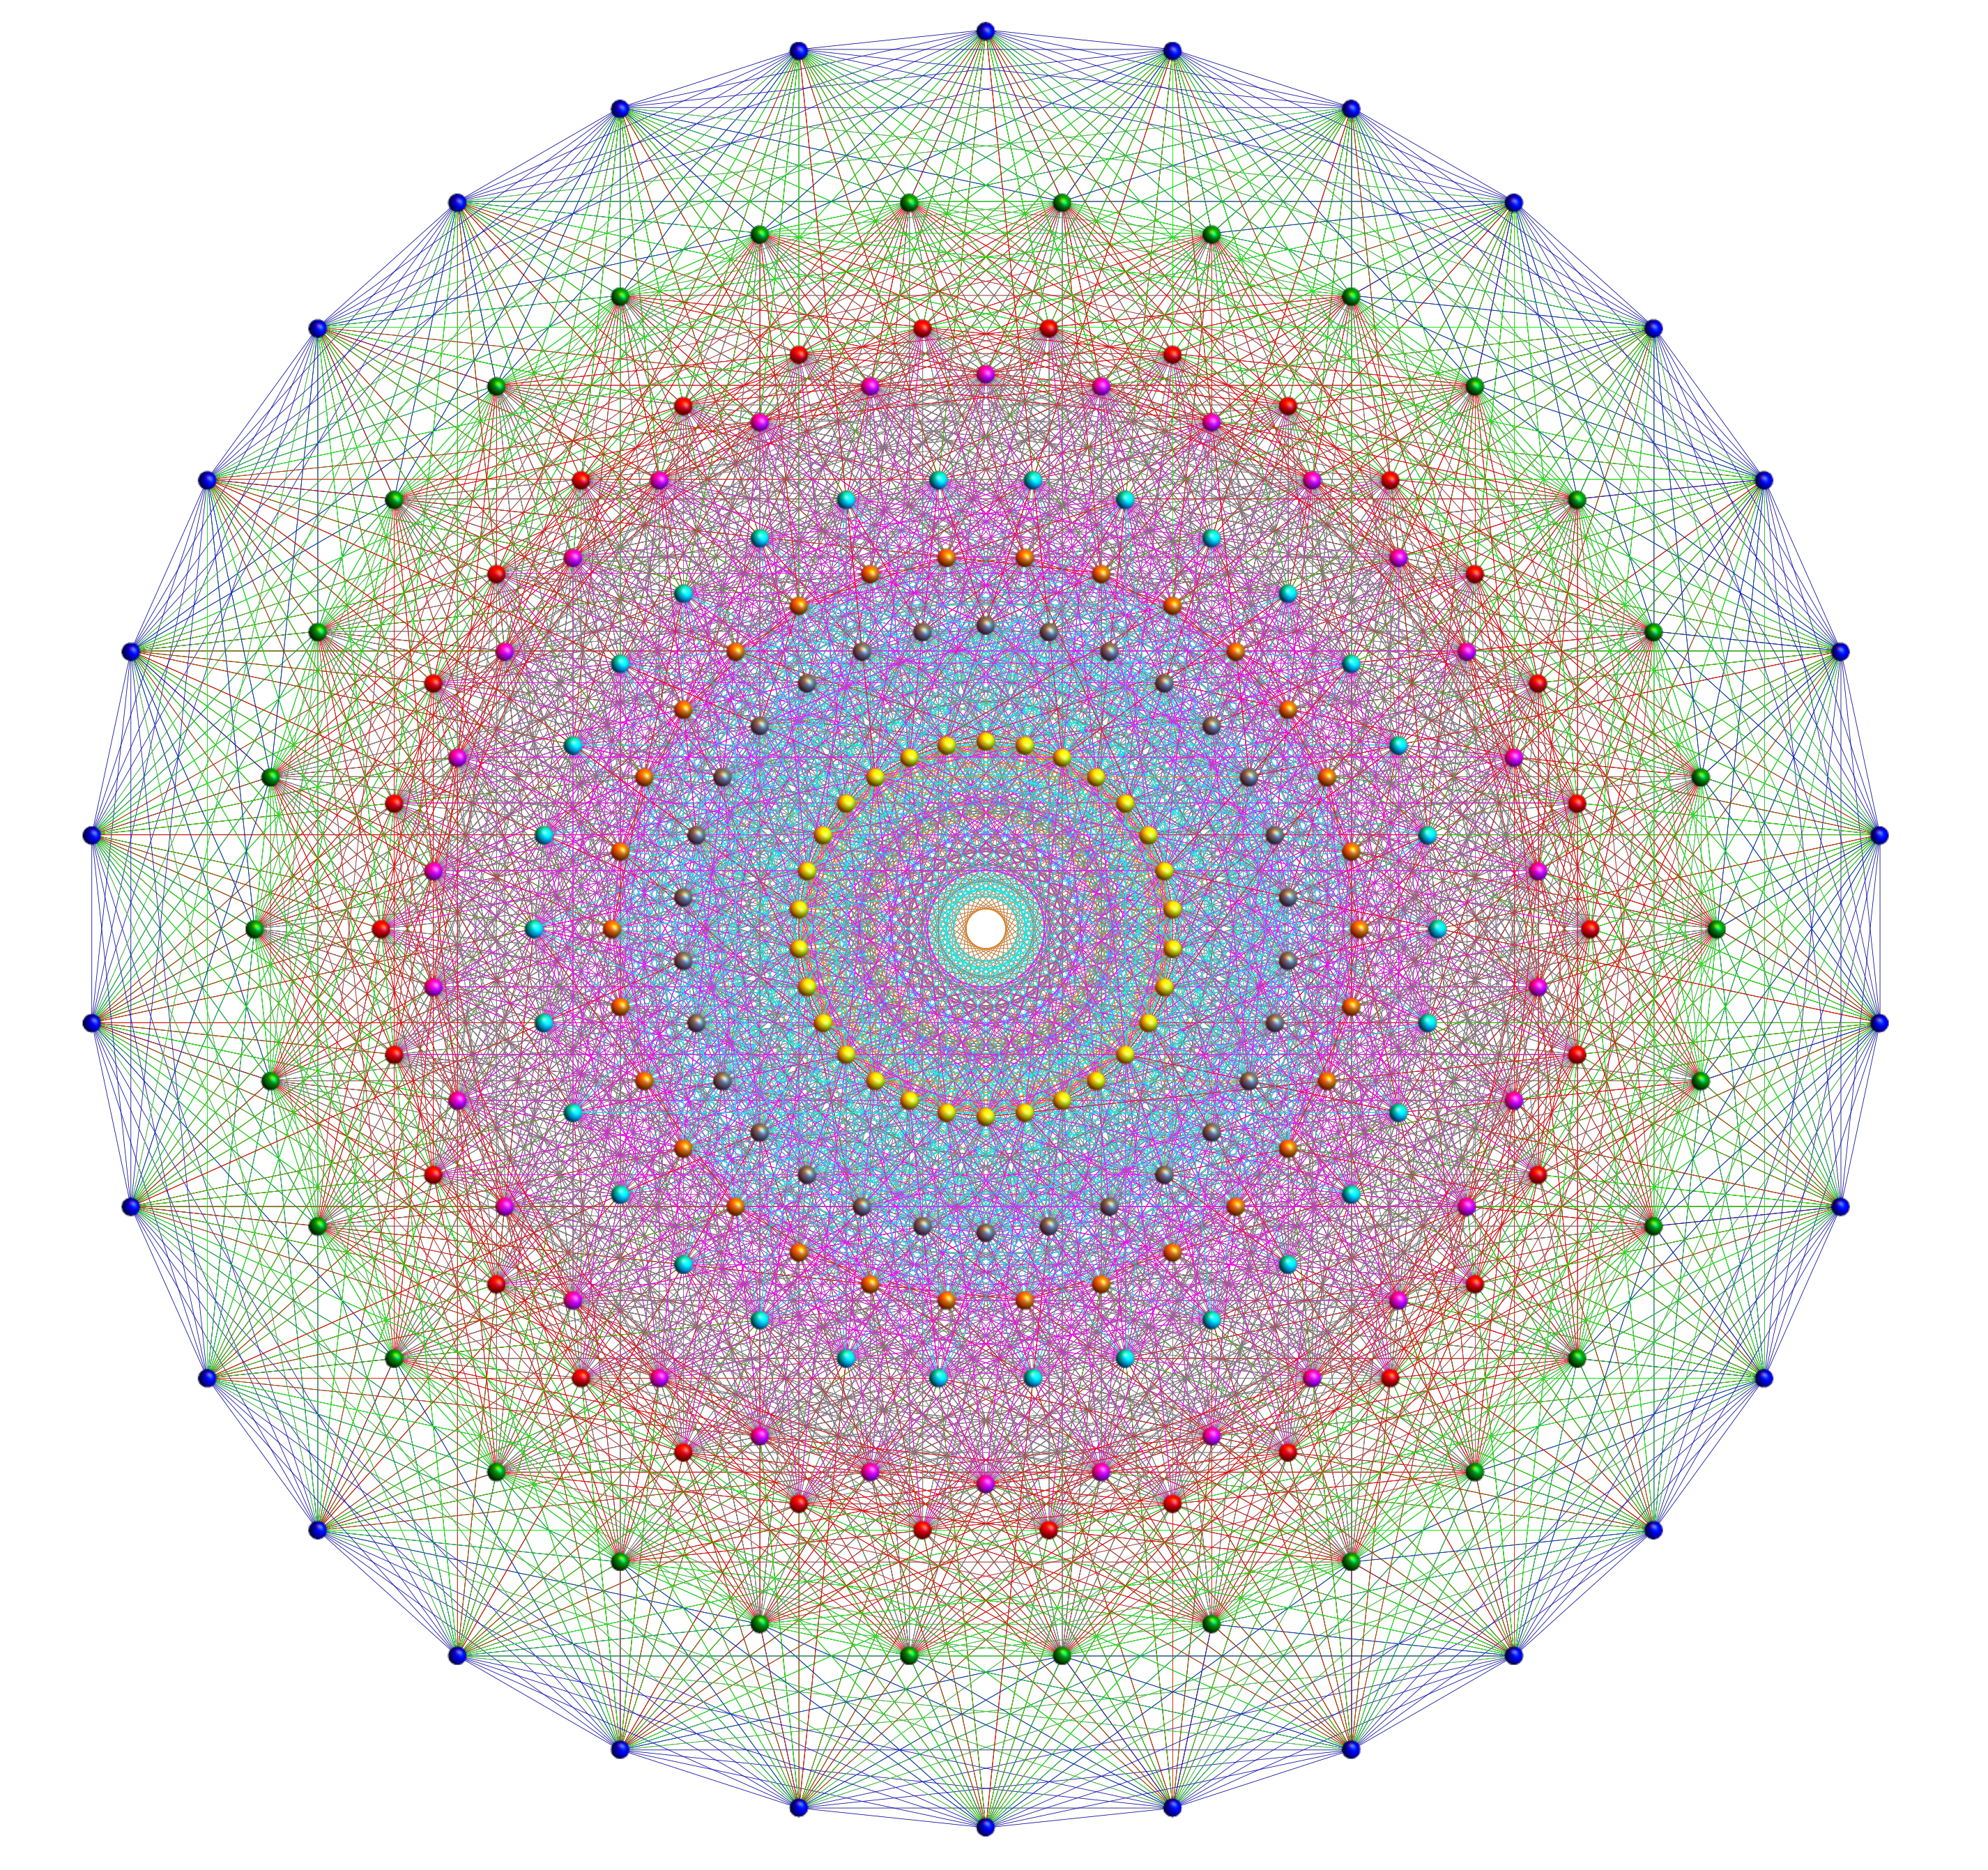
\includegraphics[width=1\columnwidth]{front.jpg}
\end{figure}

\newpage
\tableofcontents 
\newpage
\section{Spazi metrici, topologici e applicazioni continue}
\subsection{Spazi metrici}
\begin{definizione}
	{Spazio metrico}{}
Sia $X$ un insieme non vuoto; allora $X$ si dice spazio metrico se pu\`o essere equipaggiato con una \textit{distanza}, ossia una funzione $d : X \times X \to \mathbb{R}$ tale che:
\begin{itemize}
	\item $d(x,x') \ge  0 $ e $d(x,x') = 0 \iff x=x'$;
	\item $d(x,x') = d(x',x)$;
	\item $d(x,x'') \le  d(x,x') + d(x',x'')$.
\end{itemize}
\end{definizione}
\noindent Dato uno spazio metrico $(X,d_X)$ e un insieme $Y \subset  X$, si pu\`o definire un sottospazio di $(X,d_X)$ restringendo la distanza al solo $Y$:
\[
d_Y (y,y') := d_X(y,y'), \ \forall y,y' \in Y
\] 
Quindi $(Y,d_Y)$ \`e a sua volta uno spazio metrico, sottospazio di $(X,d_X)$, il quale \`e detto \textit{spazio ambiente} di $Y$.
\subsubsection{Insiemi aperti}
In uno spazio metrico $(X,d)$, si pu\`o definire un \textit{disco aperto} di raggio $r$ e centro $x$ come
\[
B_r(x) := \left\{ x' \in X  \mid d(x,x') < r \right\} 
\] 
\begin{definizione}
	{Insieme aperto}{}
	Sia $(X,d)$ uno spazio metrico. Un suo sottoinsieme si dice aperto se \`e generato dall'unione di dischi aperti.
\end{definizione}
\subsubsection{Continuit\`a in spazi metrici}
Una funzione $f:\mathbb{R}\to \mathbb{R}$ si dice continua in $x \in \mathbb{R}$ se $\forall \varepsilon , \ \exists \delta (\varepsilon )$ tale che:
\[
\lvert f(x) - f(x') \rvert < \varepsilon, \ \forall \lvert x-x' \rvert < \delta (\varepsilon )
\] 
\`E possibile generalizzare la definizione a spazi metrici usando la metrica definita su di essi.
\begin{definizione}
	{Continuit\`a in spazi metrici}{}
Sia $f : X\to Y$ un'applicazione, con $(X,d_X) , \ (Y,d_Y)$ spazi metrici. Si dice che $f$ \`e continua in $x \in X$ se $\forall \varepsilon , \ \exists \delta (\epsilon )$ tale che:
\begin{equation}
	d_Y \big(f(x), f(x')\big) < \varepsilon , \ \forall d_X(x,x')< \delta (\varepsilon )
\end{equation}
\end{definizione}
\noindent Usando la nozione di insieme aperto, \`e possibile generalizzare ulteriormente la definizione di continuit\`a al solo concetto di apertura di un insieme.
\begin{teorema}
	{}{}
Un'applicazione $f:X\to Y$ \`e continua $\iff\forall A \subset  Y$ aperto, l'insieme $f^{-1}(A)  $ \`e aperto.
\begin{proof}
Si dimostrano le due implicazioni.	
\begin{itemize}
	\item $(\Rightarrow )$ Si assume che $f$ sia continua. Si prende $f(x) \in A$, con $A\subset Y$ aperto, per qualche $x \in f^{-1} (A)$. Essendo $A$ aperto $\Rightarrow \exists \varepsilon >0 : B_\varepsilon \big(f(x)\big)\subset A$; allo stesso tempo, per continuit\`a di $f$, dato $\varepsilon $ scelto prima, deve esistere $\delta (\varepsilon )$ tale che
		\[
		f\big(B_{\delta (\varepsilon )}(x)\big) \subset B_\varepsilon \big(f(x)\big)
		\] 
	quindi $B_{\delta (\varepsilon )} (x) \subset f^{-1} (A)$. Valendo $\forall x \in f^{-1} (A)\Rightarrow f^{-1} (A)$ \`e aperto perch\'e per ogni suo elemento, esiste una palla tutta contenuta al suo interno.
\item $(\Leftarrow)$ Si assume che $\forall A \subset Y$ aperto, la funzione $f$ sia tale che l'insieme $f^{-1} (A)$ \`e aperto. Per $f(x) \in Y$, esiste $B_\varepsilon \big(f(x)\big) \subset Y$; essendo questo aperto, deve essere aperto anche $f^{-1} \big[B_\varepsilon \big(f(x)\big) \big]$. Per costruzione $x \in f^{-1} \big[B_\varepsilon \big(f(x)\big) \big] $, perci\`o $\exists \delta (\varepsilon ) : B_{\delta (\varepsilon )} (x) \subset f^{-1} \big[B_\varepsilon \big(f(x)\big) \big]$, quindi vuol dire che $f\big(B_{\delta (\varepsilon )} (x)\big)\subset B_\varepsilon \big(f(x)\big)$, ossia:
	\[
	d_Y\big(f(x), f(x')\big) < \varepsilon , \ \forall d_X (x,x') < \delta (\varepsilon )
	\] 
Valendo $\forall x \in X$, allora $f$ \`e continua.
\end{itemize}
\end{proof}
\end{teorema}
\noindent Questo permette di parlare di continuit\`a di applicazioni in insiemi su cui non \`e definita una distanza, ma solo i sottoinsiemi aperti.
\subsubsection{Distanze equivalenti}
\begin{definizione}
	{Distanze topologicamente equivalenti}{}
	Due distanze $d,\overline{d}$ su $X$ si dicono \textit{topologicamente equivalenti} se 
	\begin{equation}
		d(x,x') = r \overline{d}(x,x'), \ \text{ per qualche } r\in \mathbb{R}^{>0}
	\end{equation}
\end{definizione}
\noindent Evidentemente, $\forall \epsilon >0$:
\[
B_\varepsilon (x) = \overline{B}_{r\varepsilon } (x)
\] 
cio\`e le due distanze $d,\overline{d}$ identificano le stesse palle aperte, quindi gli stessi insiemi aperti, da qui il termine \textbf{topologicamente equivalenti}.
In $\mathbb{R}^n$, le distanze 
\begin{equation}
	\begin{split}
		&d_2(x,x') = \left\lVert x-x' \right\rVert \equiv \sqrt{\sum_{i=1}^{n} (x_i-x'_i)^2} \\
		&d_1(x,x') = \sum_{i=1}^{n} \lvert x-x_i \rvert \\
		&d_{\infty}(x,x') = \max_{i} \left\{ \lvert x_i-x'_i \rvert  \right\} 
	\end{split}
\end{equation}
sono equivalenti e si ha
\begin{equation}
	d_{\infty} (x,x') \le d_2(x,x') \le d_1 (x,x') \le n d_\infty(x,x')
\end{equation}
\begin{proof}
	La prima disuguaglianza \`e giustificata da:
	\[
	d_2 (x,x') = \sqrt{\sum_{i=1}^{n} (x_i -x'_i)^2}  \ge \sqrt{\max_i  \left\{ (x_i-x'_i)^2 \right\} } = \max_i \left\{ \lvert x-x'_i \rvert  \right\} = d_\infty(x,x')
	\] 
	La seconda, invece, \`e vera perch\'e:
	\[
	\left[ d_2(x,x') \right] ^2 = \sum_{i=1}^{n} (x-x'_i)^2 \le \left[ \sum_{i=1}^{n} \lvert x_i-x'_i \rvert  \right] ^2 = \left[ d_1(x,x') \right] 
	\] 
L'ultima disuguaglianza \`e immediata.	
\end{proof}
Da questo segue direttamente che\footnote{Apparentemente, la distanza pi\`u grande dovrebbe includere pi\`u elementi, quindi i simboli $\supset$ dovrebbero essere dei $\subset$, invece, avendo fissato il raggio $\varepsilon $, quella che permette di creare la palla pi\`u grande \`e la distanza pi\`u piccola perch\'e \textit{avvicina} i punti tra di loro, quindi pi\`u elementi rientreranno in tale raggio.}
\begin{equation}
	B^{(\infty)} _\varepsilon (x) \supset B^{(2)} _\varepsilon (x) \supset B^{(1)} _{\varepsilon } (x) \supset B^{(\infty)} _{\varepsilon  / n} (x)
\end{equation}
Questo mostra che se $A$ \`e aperto rispetto ad una distanza, lo \`e anche rispetto alle altre.
\subsubsection{Alcuni risultati sulla continuit\`a}
\begin{prop}
	{}{c11}
Siano $(X,d_X), \ (Y,d_Y)$ due spazi metrici e $f:X\to Y$ un'applicazione. Dato $x \in X$, se esiste costante $M>0$ tale che
\[
d_Y\big(f(x'), f(x)\big) \le Md_X(x',x), \ \forall x ' \in X
\] 
allora $f$ \`e continua in $x$.
\begin{proof}
	Segue direttamente dal fatto che, per ipotesi, definendo $\delta (\varepsilon ) = \varepsilon / M$, si ha $f\big(D_{\delta (\varepsilon )} (x)\big) \subset D_\varepsilon \big(f(x)\big)$.
\end{proof}
\end{prop}
\begin{prop}
	{}{c12}
	Ogni applicazione lineare $L : \mathbb{R}^n \to \mathbb{R}^m$ \`e continua rispetto alle distanze euclidee.
	\begin{proof}
		Si usa Prop. \ref{prop:c11} applicato alle distanze $d^{(1)} $, che sono topologicamente equivalenti alle distanze euclidee $d^{(2)} $. Inoltre, visto che ogni applicazione costante \`e continua, si esclude che $L$ sia nulla. Si denota con $(a_{ij} )_{1\le i\le m, \ 1\le j\le n} $ la matrice che rappresenta $L$; se $x, x' \in \mathbb{R}^n$ si ha:
		\[
			\begin{split}
				d^{(1)} \big(L(x) , L(x')\big)&= \left\lvert \sum_{j=1}^{n} a_{1j} (x_j-x'_j) \right\rvert + \ldots+ \left\lvert  \sum_{j=1}^{n} a_{mj} (x_j - x'_j) \right\rvert \\
						       &\le \left(\max_j \lvert a_{1j} \rvert+ \ldots +\max_j \lvert a_{mj}  \rvert   \right) \sum_{j=1}^{n} \lvert x_j - x'_j \rvert \le  Mm d^{(1)} (x,x')
			\end{split}
		\] 
		con $M=\max \lvert a_{ij}  \rvert$, che \`e maggiore di $0$ perch\'e $L$ \`e non-nulla. Da Prop. $\ref{prop:c11}$, segue la tesi.
	\end{proof}
\end{prop}
\noindent La precedente proposizione pu\`o essere applicata al caso particolare di applicazioni lineari: le \textbf{proiezioni}. Una proiezione \`e generalmente definita come:
\begin{equation}
	p_i:\mathbb{R}^n \to \mathbb{R}, \ p_i(x) = x_i
\end{equation}
\`E possibile definire, pi\`u in generale, per $1\le i_1 < i_2< \ldots<i_m <n$, la proiezione
\begin{equation}
	p_{i_1,\ldots,i_m}:\mathbb{R}^n \to \mathbb{R}^m, \  p_{i_1,\ldots,i_m} (x) = (x_{i_1} ,\ldots,x_{i_m} )
\end{equation}
che \`e lineare e, quindi, continua.
\subsubsection{Isometrie e omeomorfismi}
\begin{definizione}
	{Isometria}{}
	Dati $X,Y$ spazi metrici, un'applicazione biettiva $f:X\to Y$ \`e un'isometria se $\forall x,x' \in X$, si ha $d_X(x,x') = d_Y\big(f(x),f(x')\big)$.
\end{definizione}
\noindent Da Prop \ref{prop:c11}, segue che un'isometria \`e un'applicazione continua. Se fra due spazi metrici $X,Y$ esiste un'isometria $f:X\to Y$, gli spazi si dicono \textbf{isometrici}. 

Sono isometrie $\operatorname{Id} : X \to X$, cio\`e l'applicazione identit\`a, l'inversa di un'isometria e la composizione di isometrie. Questo porta al seguente.
\begin{prop}
	{}{}
	Un'isometria fra due spazi metrici \`e una relazione di equivalenza.	
\end{prop}
\begin{definizione}
	{Omeomorfismo}{}
	Dati $X,Y$ spazi metrici, un'applicazione biettiva $f:X\to Y$ \`e un \textit{omeomorfismo} se la sua inversa e $f$ stessa sono continue.
\end{definizione}
\noindent Ne segue che ogni isometria \`e un omeomorfismo, ma non \`e vero il viceversa. Per esempio, definendo $e^x : \mathbb{R} \to (0,+\infty)$, questa ha un'inversa continua $\log(x) : (0,+\infty) \to \mathbb{R}$, quindi \`e un omeomorfismo, ma non \`e un'isometria perch\'e manda $(-\infty,0]$ in $(0,1]$.

Anche gli omemorfismi definiscono una \textbf{relazione di equivalenza} tra spazi metrici.
\subsection{Spazi topologici}






























\end{document}
